

\section{Experimental Setup}

\subsection{Evaluation Platforms} We evaluate our approach on two GPU platforms.
The first platform has an NVIDIA RTX 2080Ti GPU (2080Ti), which integrates 4350 CUDA cores for floating point computation and 4350 CUDA
cores for integer operations. The GPU has a 64KB of shared memory. The host machine has a 2.30GHz Intel Xeon E5-2697 CPU with 252GB memory,
running Linux kernel v4.15.0. We use CUDA Toolkit 11.0 and cuDNN 7.6.5. The second platform has an NVIDIA Jetson AGX Xavier GPU (Xavier),
which integrates 512 Volta cores and 48KB shared memory. The host machine has an 1.2GHz 8-core ARM CPU with 32GB memory, running Linux
kernel v4.9.140-tegra. We use CUDA Toolkit 10.0 and cuDNN 7.6.3.


\subsection{Competing Methods} We compare our approach against the state-of-the-art convolution library cuDNN which supports all kinds of convolutions including depthwise and pointwise convolutions on GPU.
  Moreover, cuDNN can execute GEMM-, FFT- and Winograd-based convolutions.
%  We take cuDNN GEMM implementation as a baseline for pointwise convolution.
%  We implement a direct depthwise convolution without using the proposed reuse algorithms.
%  We take this implementation as a baseline for depthwise convolution.


\subsection{Use Cases}
We apply our approach to depthwise convolution and pointwise convolution, described as follows.

\mypara{Depthwise convolution.} This applies a bank of single-channel 2D filters to convolve with one multi-channel 2D input, e.g., an image of three color channels, R, G and B. We apply a 2D convolution filter to each of the input channels.
This technique has been widely used in many CNNs, including MobileNetv2 \cite{Sandler_2018_CVPR}, EfficientNet \cite{tan2019efficientnet} and ShuffleNetv2 \cite{Ma_2018_ECCV}.

\mypara{Pointwise convolution.} This applies a bank of multi-channel 2D 1$\times$1 filters to convolve with one multi-channel 2D input.
The 2D convolution is performed between one filter channel and the corresponding input channel, and the results are sum up across channels to generate one output channel.


\subsection{Performance Report}
We run each test case ten times with batch sizes 1, 8, 16, 32, 64 and 128 on an unloaded machine and report the averaged running time.
We found little variance during execution runs, less than 2\%.
We run convolutions with two data types, 32bit floating point (FP32) for normal CNNs and 8bit integer (INT8) for quantized CNNs.
In our experiments, we utilize $NCHW$ for FP32 and $NHWC$ for INT8.

In this work, we first test depthwise convolution with two filter sizes, $3 \times 3$ and $5 \times 5$, because these are commonly used filter sizes.
Then we report the performance of pointwise convolution.
Lastly, we apply our optimized depthwise and pointwise convolutions on normal and quantized MobileNetv2 and report the performance of inference and training.
%
%\subsection{Notations}
%Throughout the evaluation, we use $I$, $F$, and $O$ to represent the input, the filter, and the output respectively, $N$, $C$, $H$, and $W$
%to denote the batch size, the channel, the height, and the width, respectively.

\section{Experimental Results}
\label{exp} In this section, we report results for depthwise convolution (Section \ref{sec:depconvexp}), pointwise convolution (Section \ref{sec:pwconvexp}) and inference and training of MobileNetV2 (Section \ref{sec:inferexp}), showing that our approach consistently outperforms alternative methods by delivering the overall best performance.


%\subsection{2D Convolution\label{sec:ex2dc}}
%\begin{figure*}
%\centering
%\subfloat[][$3 \times 3$ filter]{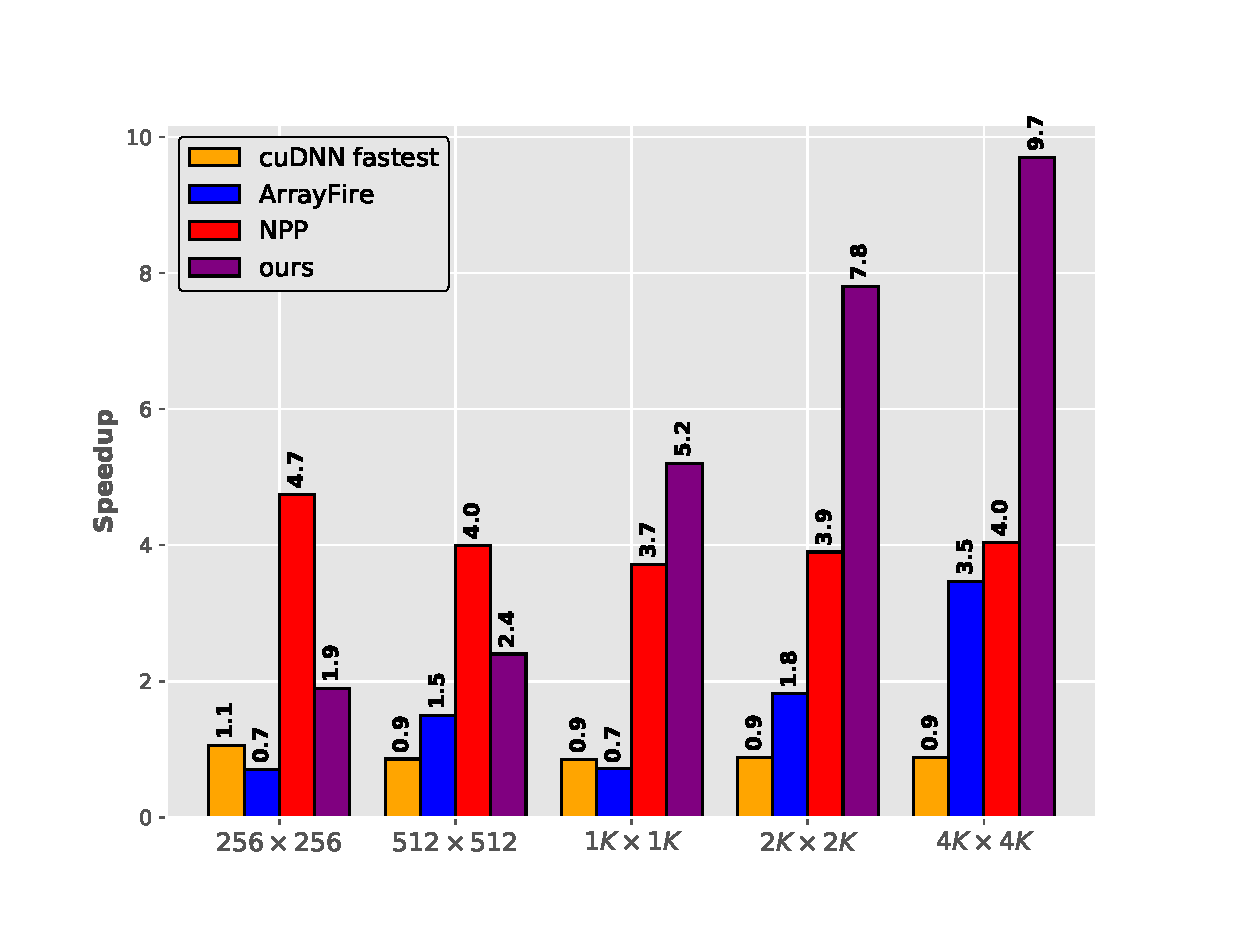
\includegraphics[width=0.85\columnwidth]{./figure/2d_conv_f3.eps}
%	\label{fig:2druntimef3c12080}}
%\hspace{0em}
%\subfloat[][$5 \times 5$ filter]{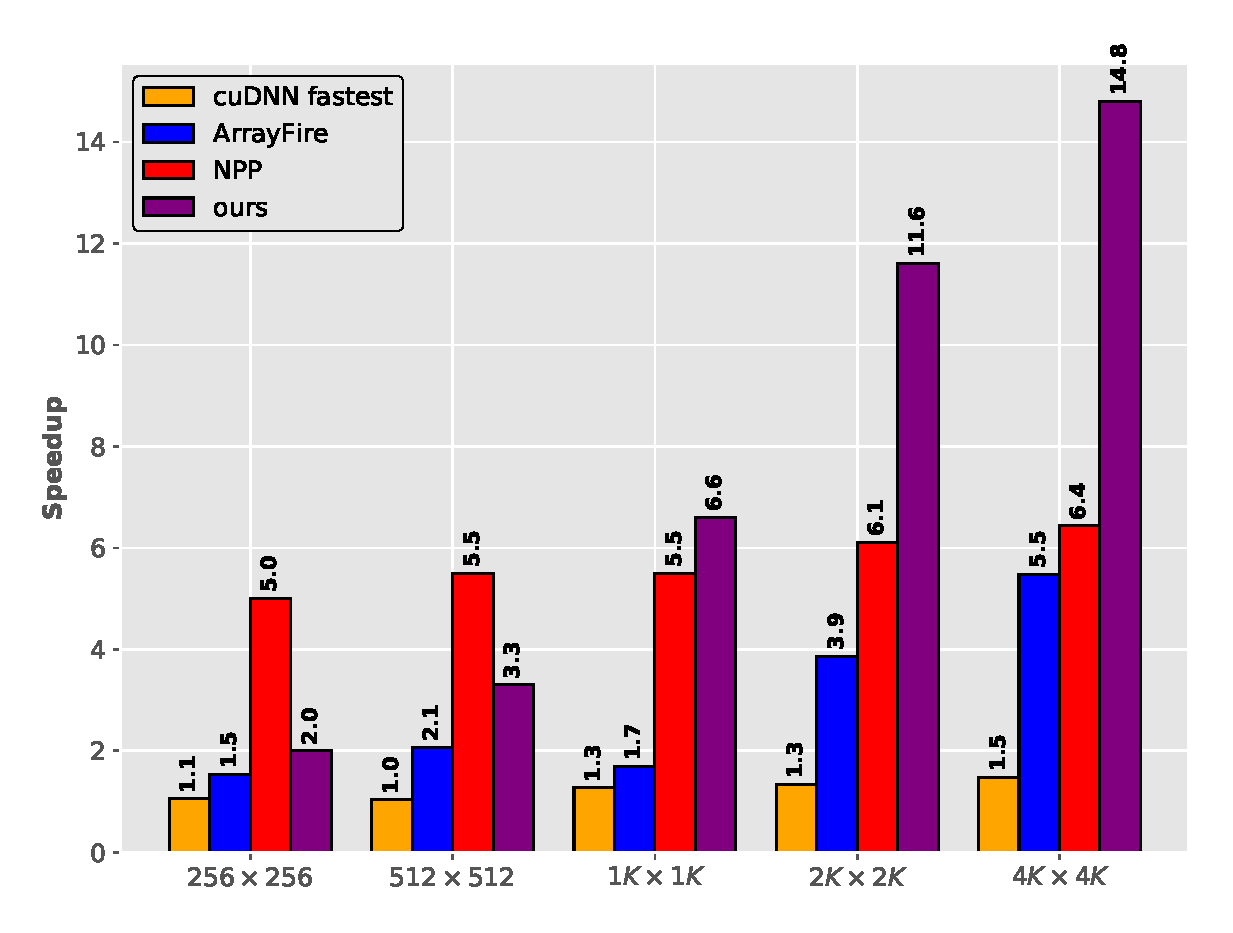
\includegraphics[width=0.85\columnwidth]{./figure/2d_conv_f5.eps}
%	\label{fig:2druntimef5c12080}}
%
%\vspace{-1mm}	\caption{Speedups of 2D convolutions of four implementations over GEMM-im2col when using a $3 \times 3$ (a) and a $5 \times
%5$ filter (b).} \label{fig:2druntime} \vspace{-3mm}
%\end{figure*}
%
%
%\subsubsection{Setup}
%In this experiment, we compare our approach against the 2D convolution implementations from cuDNN, GEMM-im2col, ArrayFire, and
%NPP. As cuDNN provides multiple implementations, we empirically choose the fastest version, denoted as cuDNN-fastest, for evaluation. We
%apply each method to images with sizes ranging from $256 \times 256$ to $4K \times 4K$. We set the batch size, channel, height, and width
%of the input to be 1.
%
%
%\subsubsection{Overall results}
% Figure
%\ref{fig:2druntime} reports the speedups of cuDNN, ArrayFire, NPP and our approach over GEMM-im2col. While cuDNN has been heavily optimized
%for NVIDIA GPUs, it does not show a notable performance advantage. When using a $3 \times 3$ filter, our approach gives the best overall
%speedup of 5.4$\times$ (up to 9.7$\times$ for the largest input), which translates to an improvement of  more than 30\% over the second-best method, NPP.
%We note that our approach is based on the standard 2D direct convolution by applying the column and row reuse algorithms. Therefore, the
%performance gain is mainly attributed to the reduction of the number of memory transactions. When using a $5 \times 5$ filter, our approach
%achieves a better overall speedup of $7.7\times$. A $5 \times 5$ filter has four overlapped columns and rows (instead of just one
%overlapped column and row on width and height dimensions when using a $3 \times 3$ filter). The larger number of overlapped data thus gives
%more room for performance optimization when using our column and row reuse algorithms. Our approach achieves the best overall performance
%and demonstrates significant performance advantages when processing large input.
%
%\subsubsection{Further analysis}
%\begin{figure}[t!]
%\centering
%
%\subfloat[][Memory throughput]{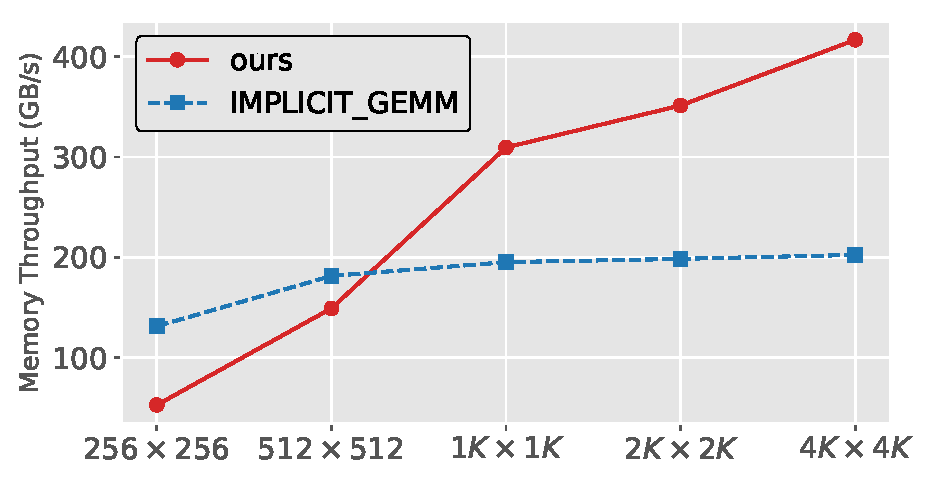
\includegraphics[width=0.85\columnwidth]{./figure/2dmemthroughput.eps}
%	\label{fig:2dmemthr}}
%
%\subfloat[][Maximum bandwidth]{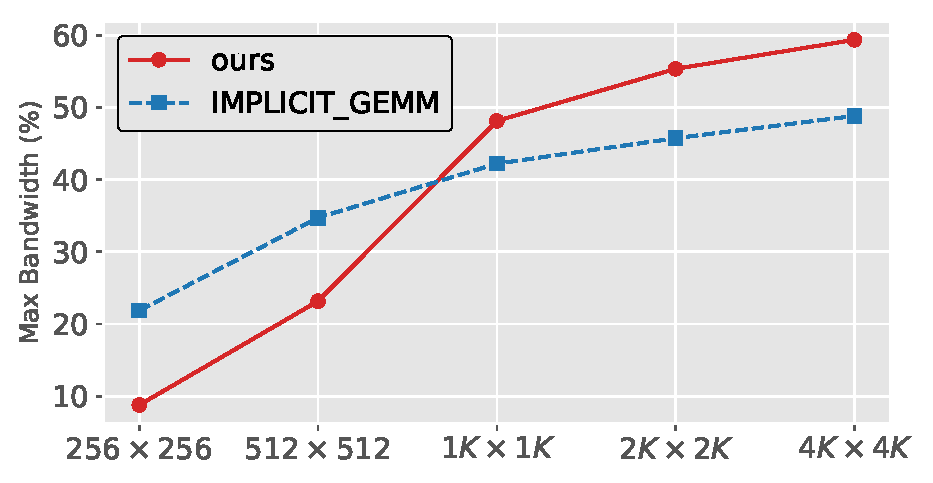
\includegraphics[width=0.85\columnwidth]{./figure/2dmembandwidth.eps}
%	\label{fig:2dmaxband}}
%	
%\caption{Memory throughput (a) and maximum bandwidth (b) of NPP and our implementation for the filter of size $3 \times 3$.}
%\label{fig:2dmemanaly}
%\vspace{-5mm}
%\end{figure}
%
%On the test cases of small input sizes (i.e., $256 \times 256$ and $512 \times 512$), NPP gives the best performance. To understand the
%performance gap on small input sizes, we use \emph{nvidia compute} to collect memory profiles, including memory throughput and max
%bandwidth, of our implementation and NPP when using a $3 \times 3$ filter to perform convolution. The profiling results are shown in Figure
%\ref{fig:2dmemanaly}.  We see that as the input size increases, the memory throughput and the maximum bandwidth also grow. This is expected
%as the larger the input image, the larger number the memory transactions is likely to be when performing convolution.  We also observe that
%our approach leads to higher memory throughput and the maximum bandwidth used when the input image size is greater or equal than $1K \times
%1K$. This finding matches the results presented in Figure \ref{fig:2druntime}, where our approach gives the best performance when
%processing an image whose size is $1K \times 1K$ or larger. This result also suggests that memory performance has a strong correlation with
%the performance of 2D convolutions.
%
%
%The reason why our approach gives lower memory throughput and achieves lower maximum bandwidth on small input sizes over NPP is explained
%as follows. For 2D convolution, only one filter is used to convolve with one single-channel input feature map, which
%requires much less computation compared to, e.g., the depth-wise or multi-channel 2D convolutions. Therefore, memory performance has a huge
%impact on the performance of 2D convolutions. Our row reuse algorithm performs better when a thread operates on more rows of output.
%However, the more rows a thread compute on, the fewer warps and thread blocks we can generate. Without enough warps issuing memory
%requests, the memory throughput and maximum bandwidth will reduce significantly, which leads to slower performance over NPP. As the input
%size increases, we can allocate more thread blocks and more warps per thread block. With enough memory requests and a reduction in redundant
%memory transactions, we can increase the memory throughput and max bandwidth to improve the performance of 2D convolutions.
%
%\subsubsection{Summary} Overall, our optimization algorithms can greatly reduce the number of memory transactions and improve the performance of 2D
%convolutions. Compared with state-of-the-art image processing libraries, NPP, our approach achieves average speedups of 1.4$\times$ and
%1.3$\times$ when using a $3 \times 3$ and $5 \times 5$ filters, respectively.

\subsection{Depthwise Convolution}
\label{sec:depconvexp}

\begin{table}[]
\caption{Layer configurations of depthwise  convolutions.}
\vspace{-3mm}
\label{tab:depconvconfigs}
\centering
\rowcolors{2}{}{Gray}
\begin{threeparttable}
\begin{tabular}{lrrrrr}
\toprule
& \textbf{$I_N$} & \textbf{$I_C$} & \textbf{$I_H \times I_W$ }&  \textbf{$F_H \times F_W$} &\textbf{$S$}\\
\midrule
\textbf{CV1} & 1,8,16,32,64,128  & 16    & 112$\times$112 & $3 \times 3$, $5 \times 5$&2  \\
\textbf{CV2} & 1,8,16,32,64,128  & 72    & 56$\times$56  &$3 \times 3$, $5 \times 5$  &2 \\
\textbf{CV3} & 1,8,16,32,64,128  & 88   & 28$\times$28  &$3 \times 3$, $5 \times 5$   &1 \\
\textbf{CV4} & 1,8,16,32,64,128  & 96    & 28$\times$28  &$3 \times 3$, $5 \times 5$  &2  \\
\textbf{CV5} & 1,8,16,32,64,128  & 96   & 14$\times$14  &$3 \times 3$, $5 \times 5$   &1 \\
\textbf{CV6} & 1,8,16,32,64,128  & 120   & 14$\times$14  &$3 \times 3$, $5 \times 5$  &1  \\
\textbf{CV7} & 1,8,16,32,64,128  & 192   & 14$\times$14  &$3 \times 3$, $5 \times 5$  &1  \\
\textbf{CV8} & 1,8,16,32,64,128  & 240   & 14$\times$14  &$3 \times 3$, $5 \times 5$  &2  \\
\textbf{CV9} & 1,8,16,32,64,128  & 432   & 7$\times$7  &$3 \times 3$, $5 \times 5$    &1\\

\bottomrule
\end{tabular}
\end{threeparttable}

\end{table}

\begin{figure*}[!t]
\centering
\subfloat[Speedups on 2080Ti for the $3 \times 3$ fitler.]{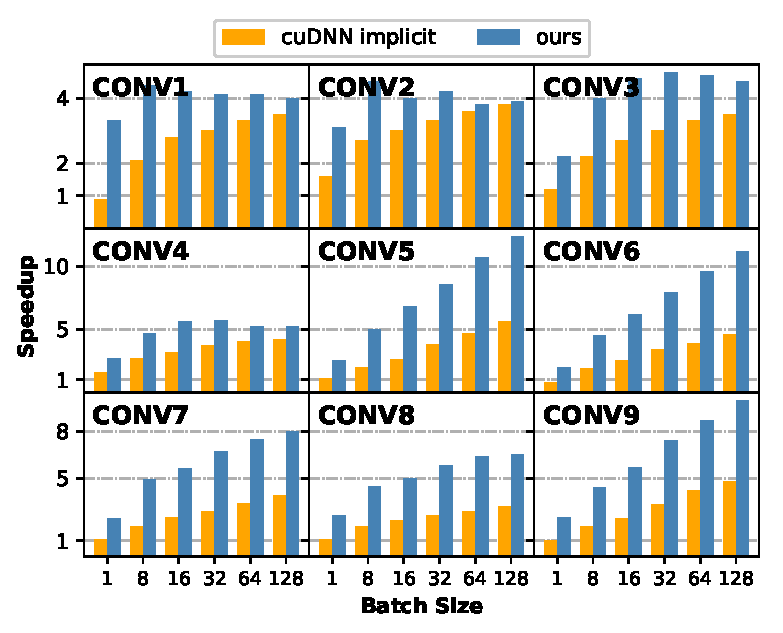
\includegraphics[width=0.4\textwidth,height=5.5cm]{./figure/dwspeeduprtxf3.eps}
	\label{fig:dwspeeduprtxf3}}
\hspace{0em}
\subfloat[Speedups on 2080Ti for the $5 \times 5$ fitler.]{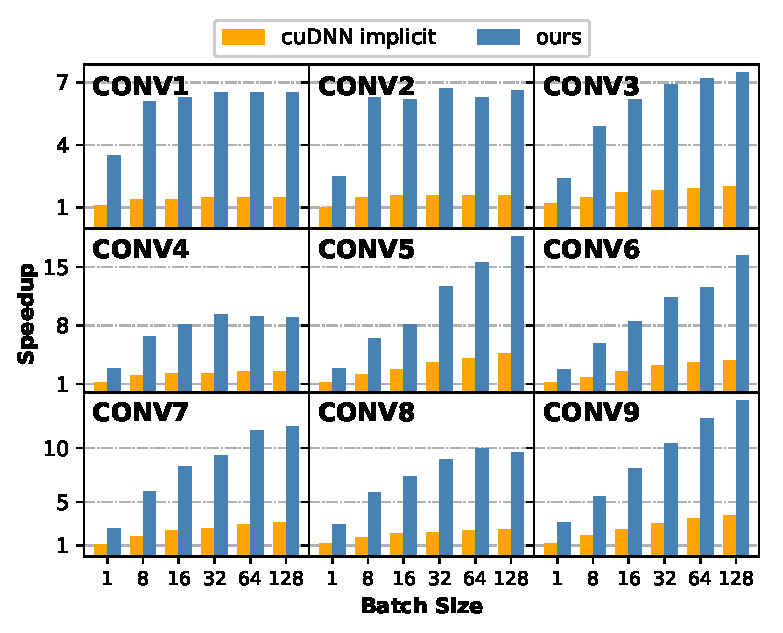
\includegraphics[width=0.4\textwidth,height=5.5cm]{./figure/dwspeeduprtxf5.eps}
	\label{fig:dwspeeduprtxf5}}
\hspace{0em}
\subfloat[Speedups on Xavier for the $3 \times 3$ fitler.]{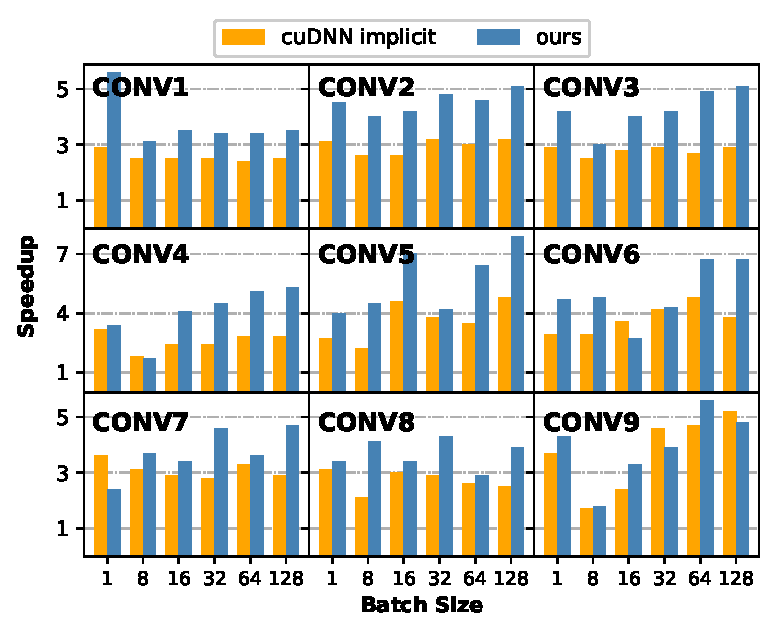
\includegraphics[width=0.4\textwidth,height=5.5cm]{./figure/dwspeedupjetsonf3.eps}
	\label{fig:dwspeedupjetsonf3}}
\hspace{0em}
\subfloat[Speedups on Xavier for the $5 \times 5$ fitler.]{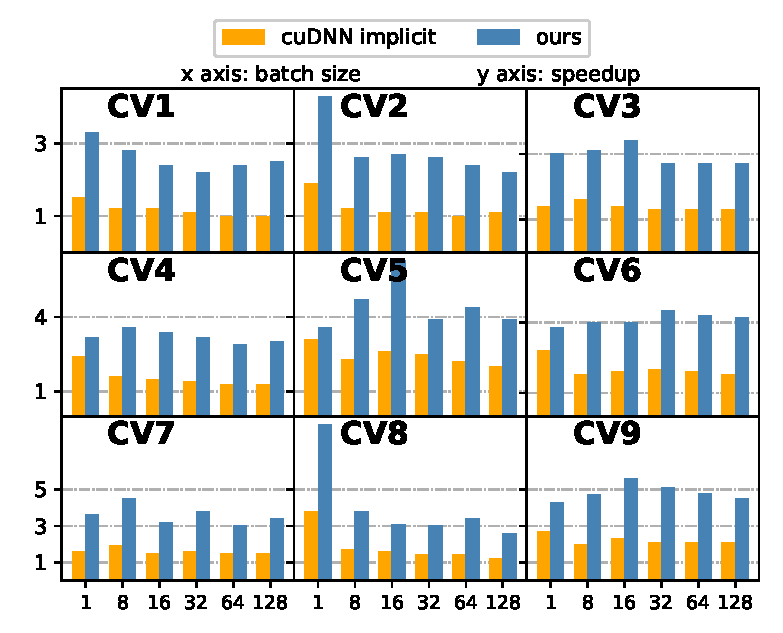
\includegraphics[width=0.4\textwidth,height=5.5cm]{./figure/dwspeedupjetsonf5.eps}
	\label{fig:dwspeedupjetsonf5}}
\caption{Speedups of cuDNN implicit and ours over the baseline implementation for depthwise convolution with filters of size $3 \times 3$ and $5 \times 5$ on two platforms.} \label{fig:dwspeedup}
\end{figure*}


%\begin{figure*}
%\centering
%	
%\subfloat[][$3\times 3$ filter]{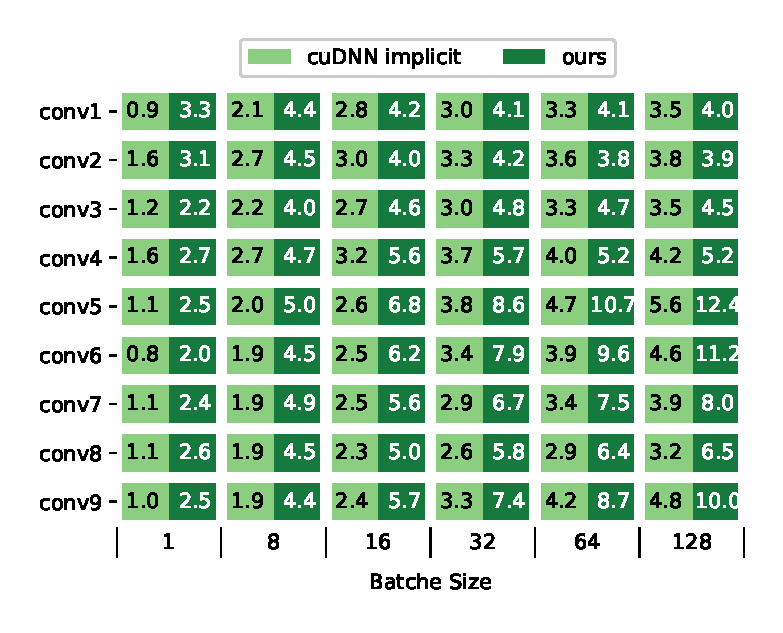
\includegraphics[width=\columnwidth]{./figure/depthwise_speedup_3f.eps}
%	\label{fig:f3dwruntime2080}}
%\subfloat[][$5\times 5$ filter]{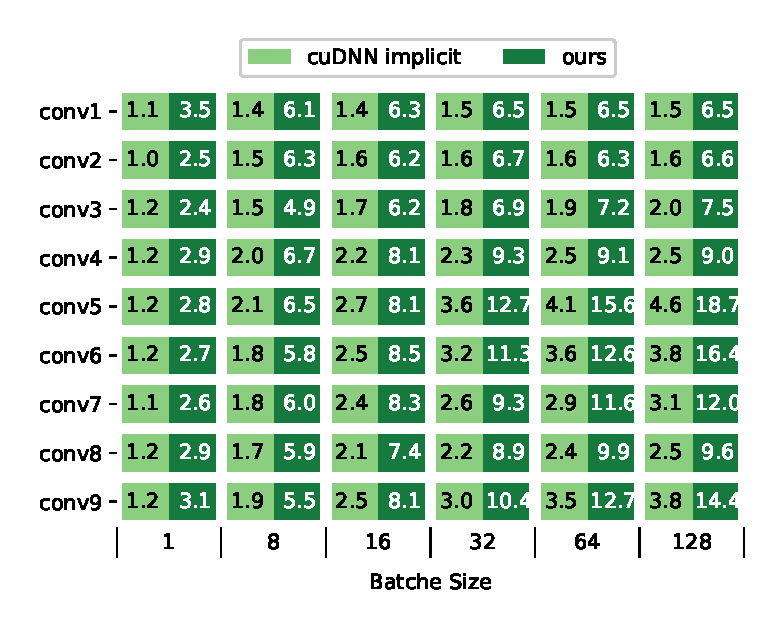
\includegraphics[width=\columnwidth]{./figure/depthwise_speedup_5f.eps}
%	\label{fig:f5dwruntime2080}}
%
%\vspace{-2mm} \caption{Speedups of our approach and cuDNN implicit algorithm over the baseline implementation of the depthwise convolution when using a
%$3\times 3$ (a) and a $5\times 5$ filter (b).} \label{fig:dwruntime}
%\vspace{-2mm}
%\end{figure*}


\subsubsection{Setup} In this experiment, we compare our approach against the depthwise convolution implementations of cuDNN. Specifically, we compare to seven algorithms in cuDNN, including IMPLICIT\_GEMM (implicit), IMPLICIT\_PRECOMP\_GEMM (precomp), GEMM (gemm), FFT (fft), FFT\_TILING (tiling), WINOGRAD (winograd) and WINOGRAD\_NONFUSED (nonfused).
As the fastest algorithm of cuDNN is always implicit, we only report the performance of the implicit algorithm for cuDNN.
We implement a simple depthwise convolution as a baseline implementation.
We use the convolutional layer configurations that apply depthwise convolution from the popular CNN model, MobileNetv2.
We report the performance when batch sizes are set to 1, 8, 16, 32, 64 and 128.
Table \ref{tab:depconvconfigs} gives the layer configurations used in this experiment.

%In the depth-wise convolution, one input element only needs to be convolved with one filter, while in the multi-channel 2D convolution, one input element needs to be convolved with all filters.
%Therefore, depth-wise convolutions require much less computation than multi-channel 2D convolutions, which makes depth-wise convolutions more sensitive to memory performance.
%Nowadays, depth-wise convolutions have been widely used in embedded CNNs, including MobileNetv2 \cite{Sandler_2018_CVPR}, EfficientNet \cite{tan2019efficientnet} and ShuffleNetv2 \cite{Ma_2018_ECCV}.
%In this section, we present the performance comparison of the depth-wise convolution between cuDNN and our implementation.
%We implement a simple depth-wise convolution and report speedups of cuDNN and our implementation over the simple depth-wise convolution.
%We evaluate 7 algorithms in cuDNN, including IMPLICIT\_GEMM (implicit), IMPLICIT\_PRECOMP\_GEMM (precomp), GEMM (gemm), FFT (fft), FFT\_TILING (tiling), WINOGRAD (winograd) and WINOGRAD\_NONFUSED (nonfused).
%Winograd can not be applied on a $5 \times 5$ filter, thus we set speedups for this algorithm to 0.
%We collect configurations of the convolutional layers using depth-wise convolution from three popular mobile embedded models,
%namely, MobileNetv2, ShuffleNetv2 and EfficientNet.
%Then, we set the number of the batch size to 512 ($I_N=O_N=512$). Other batch sizes demonstrate a similar performance because all tested implementations have a linear scale as the batch size. The exact configuration is presented in Table \ref{tab:3dconvconfigs}.

\subsubsection{Overall results}
When testing depthwise convolutions with INT8, our implementations with INT8 and cuDNN implementations with FP32 both achieve more than $10\times$ speedups over cuDNN implementations with INT8 for configurations in Table \ref{tab:depconvconfigs}.
We attribute the poor performance of cuDNN depthwise convolutions with INT8 to internal implementation issues.
Thus, we only report the performance of depthwise convolutions with FP32.

Figure \ref{fig:dwspeedup} shows that our approach gives the best speedups in almost all test cases.
Our approach delivers an average speedup of $5.4\times$ and $4.3\times$ for the $3 \times 3$ filter on 2080Ti and Xavier respectively, and $7.8\times$ and $2.2\times$ for the $5 \times 5$ filter on 2080Ti and Xavier respectively.
The cuDNN implicit algorithm achieves an average speedup of $2.8\times$ and $3.1\times$ for the $3 \times 3$ filter on 2080Ti and Xavier respectively, and $2.2\times$ and $1.7\times$ for the $5 \times 5$ filter on 2080Ti and Xavier respectively.
Other algorithms of cuDNN perform poorly in all test cases.
Since that cuDNN is a closed source, we cannot investigate the source code for further analysis.
We hypothesize that FFT- and Winograd- based algorithms focus on the reduction of computation and trades memory performance for speed.
Precomp and gemm algorithms need extra memory operations to compute output elements.
Moreover, depthwise convolution is more sensitive to memory performance than pointwise and multi-channel 2D convolutions.
Consequently, these algorithms are not suitable for depthwise convolutions.
Overall, our approach improves cuDNN implicit by $2.0\times$ and $1.4\times$ when using a $3 \times 3$  filter on 2080Ti and Xavier respectively, and $3.5\times$ and $2.1\times$ when using a $5 \times 5$ filter on 2080Ti and Xavier respectively.
%When using a $5 \times 5$ filter, our approach achieves a better overall speedup of $7.7\times$. A $5 \times 5$ filter has four overlapped columns and rows (instead of just one
%overlapped column and row on width and height dimensions when using a $3 \times 3$ filter). The larger number of overlapped data thus gives
%more room for performance optimization when using our column and row reuse algorithms.
%The algorithms of cuDNN except implicit algorithm perform poorly in all test cases and the speedups of these algorithms all below 1.
%Considering that cuDNN is a closed source, we can only guess that FFT- and Winograd- based algorithms focus on reduction of computation and
%trades memory performance for speed. Precomp and gemm algorithms need extra memory operations to compute output elements. Moreover,
%depth-wise convolution is more sensitive to memory performance than multi-channel 2D convolution. Consequently, these algorithms perform
%poorly on depth-wise convolutions.
\begin{figure}
    \centering
    \subfloat[][SM utilizations of cuDNN implicit algorithm and our approach.]{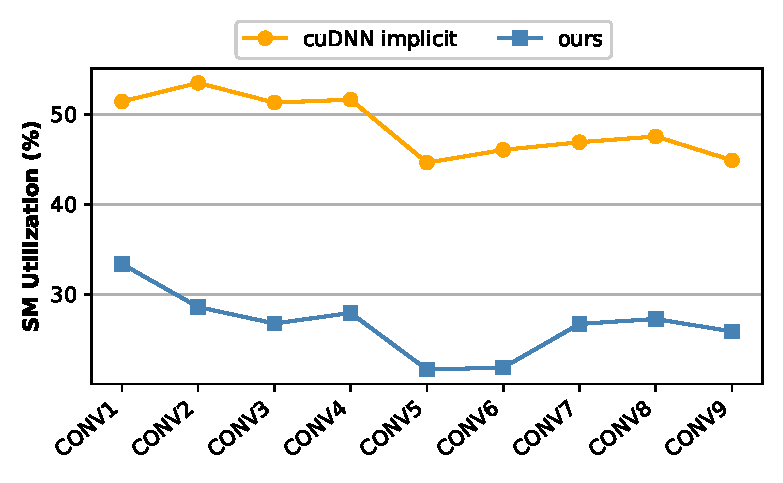
\includegraphics[width=0.9\columnwidth]{./figure/smutil.eps}\label{fig:dwsmutil}}
    \qquad
    %\vspace{5mm}
    \subfloat[][Ratios of executed LDG (load from global memory) instruction counts of cuDNN implicit algorithm to our approach.]{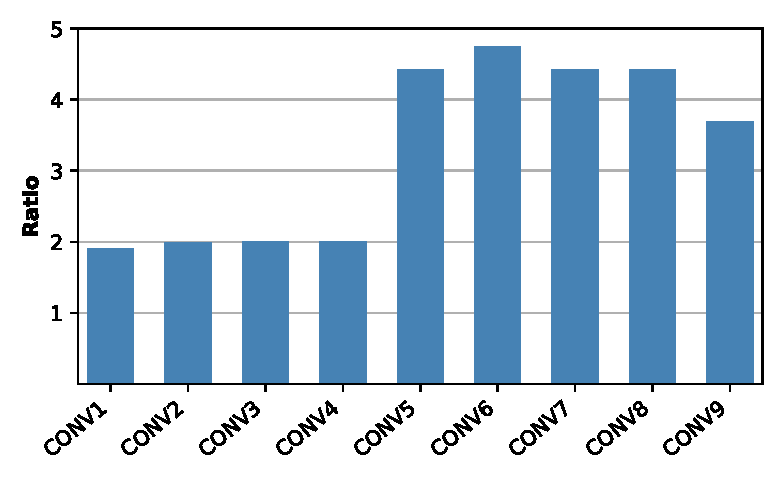
\includegraphics[width=0.9\columnwidth]{./figure/ldginst.eps}\label{fig:dwldginst}}
    \vspace{-2mm}
    \caption{SM utilization and LDG instruction counts of depthwise convolutions with a batch size of 32 and a filter size of $3\times3$ on 2080Ti.}
    \label{fig:dwratio}
\end{figure}

\subsubsection{Further analysis}
We note that our approach is based on the standard 2D direct convolution by applying the column and row reuse algorithms.
Therefore, the performance gain is mainly attributed to the reduction of the number of memory operations.

Figure \ref{fig:dwratio} reports the measured LDG (load from global memory) instruction counts and SM utilization for the fast cuDNN implicit algorithm and our approach when using a $3 \times 3$ filter and a batch size of 32 on 2080Ti. Other configurations have a similar performance.
We can see in Figure \ref{fig:dwsmutil} that cuDNN implicit algorithm has an average of $2\times$ higher SM utilization compared to our approach.
The reason why our approach gives lower SM utilization is explained as follows.
Our row reuse algorithm performs better when a thread operates on more rows of output.
However, the more rows a thread compute on, the fewer warps and thread blocks we can generate. Without enough warps running on SMs, the SM utilization will degrade significantly.
Though cuDNN implicit has high SM utilization, it does not achieve good performance for depthwise convolution.
The reason is that depthwise convolution possesses a very low computational workload and is more sensitive to memory performance.
Different from cuDNN implicit, we focus on optimizing memory performance for depthwise convolution. We use row and column reuse techniques to reduce memory operations by a maximum of $4.5\times$ lower executed LDG instructions, as shown in Figure \ref{fig:dwldginst}.
This suggests that our reuse algorithms can improve memory performance significantly, which thus leads to better overall performance.

\subsubsection{Summary}
Our approach can reduce the number of memory operations and improve memory performance, which leads to faster computation time when performing depthwise convolutions.
Compared to the fastest available algorithms in cuDNN, our approach achieves an average speedup of $2.8\times$ and $1.8\times$ when performing depthwise convolutions on 2080Ti and Xavier, respectively.


\subsection{Pointwise Convolution}
\label{sec:pwconvexp}

\begin{table}[]
\setlength{\tabcolsep}{5.2pt}
\caption{Layer configurations of pointwise convolutions.}
\vspace{-3mm}
\label{tab:pwconv}
\rowcolors{2}{}{Gray}
\begin{threeparttable}
\begin{tabular}{lrrrrr}
\toprule
& \textbf{$I_N$} & \textbf{$I_C=F_C$} & \textbf{$I_H \times I_W$} & \textbf{$F_N \times F_H \times F_W$} \\
\midrule
\textbf{CV1}  & 1,8,16,32,64,128  & 16    & $56\times 56$   & $8 \times 1\times 1$\\
\textbf{CV2}  & 1,8,16,32,64,128  & 8     & $56\times 56$   & $16 \times 1\times 1$\\
%\textbf{CONV3}  & 1,8,16,32,64,128  & 16    & $56\times 56$   & 16  & $1\times 1$\\
\textbf{CV3}  & 1,8,16,32,64,128  & 16    & $56\times 56$   & $72 \times 1\times 1$\\
\textbf{CV4}  & 1,8,16,32,64,128  & 72    & $28\times 28$   & $24 \times 1\times 1$\\
%\textbf{CONV6}  & 1,8,16,32,64,128  & 24    & $28\times 28$   & 88  & $1\times 1$\\
%\textbf{CONV7}  & 1,8,16,32,64,128  & 88    & $28\times 28$   & 24  & $1\times 1$\\
\textbf{CV5}  & 1,8,16,32,64,128  & 24    & $28\times 28$   & $96 \times 1\times 1$\\
\textbf{CV6}  & 1,8,16,32,64,128  & 96    & $14\times 14$   & $24 \times 1\times 1$\\
\textbf{CV7} & 1,8,16,32,64,128  & 24    & $14\times 14$   & $96  \times 1\times 1$\\
%\textbf{CONV11} & 1,8,16,32,64,128  & 96    & $14\times 14$   & 32  & $1\times 1$\\
\textbf{CV8} & 1,8,16,32,64,128  & 32    & $14\times 14$   & $192 \times 1\times 1$\\
\textbf{CV9} & 1,8,16,32,64,128  & 192   & $14\times 14$   & $48  \times 1\times 1$\\
%\textbf{CONV14} & 1,8,16,32,64,128  & 48    & $14\times 14$   & 192 & $1\times 1$\\
%\textbf{CONV15} & 1,8,16,32,64,128  & 192   & $14\times 14$   & 32  & $1\times 1$\\
%\textbf{CONV16} & 1,8,16,32,64,128  & 32    & $14\times 14$   & 96  & $1\times 1$\\
\textbf{CV10} & 1,8,16,32,64,128  & 96    & $14\times 14$   & $40 \times 1\times 1$\\
\textbf{CV11} & 1,8,16,32,64,128  & 40    & $14\times 14$   & $120 \times 1\times 1$\\
\textbf{CV12} & 1,8,16,32,64,128  & 120   & $14\times 14$   & $32 \times 1\times 1$\\
%\textbf{CONV20} & 1,8,16,32,64,128  & 32    & $14\times 14$   & 120 & $1\times 1$\\
%\textbf{CONV21} & 1,8,16,32,64,128  & 120   & $14\times 14$   & 40  & $1\times 1$\\
\textbf{CV13} & 1,8,16,32,64,128  & 40    & $14\times 14$   & $240 \times 1\times 1$\\
\textbf{CV14} & 1,8,16,32,64,128  & 240   & $7\times 7$     & $64  \times 1\times 1$\\
\textbf{CV15} & 1,8,16,32,64,128  & 64    & $7\times 7$     & $240 \times 1\times 1$\\
%\textbf{CONV25} & 1,8,16,32,64,128  & 240   & $7\times 7$     & 72  & $1\times 1$\\
\textbf{CV16} & 1,8,16,32,64,128  & 72    & $7\times 7$     & $432 \times 1\times 1$\\
\textbf{CV17} & 1,8,16,32,64,128  & 432   & $7\times 7$     & $112 \times 1\times 1$\\
\textbf{CV18} & 1,8,16,32,64,128  & 112   & $7\times 7$     & $432 \times 1\times 1$\\
\textbf{CV19} & 1,8,16,32,64,128  & 432   & $7\times 7$     & $72 \times 1\times 1$\\
\textbf{CV20} & 1,8,16,32,64,128  & 432   & $7\times 7$     & $1024 \times 1\times 1$\\

\bottomrule
\end{tabular}
\end{threeparttable}
\end{table}

\begin{figure*}
\captionsetup[subfloat]{labelformat=empty,skip=0pt}
	\centering
	\subfloat[]{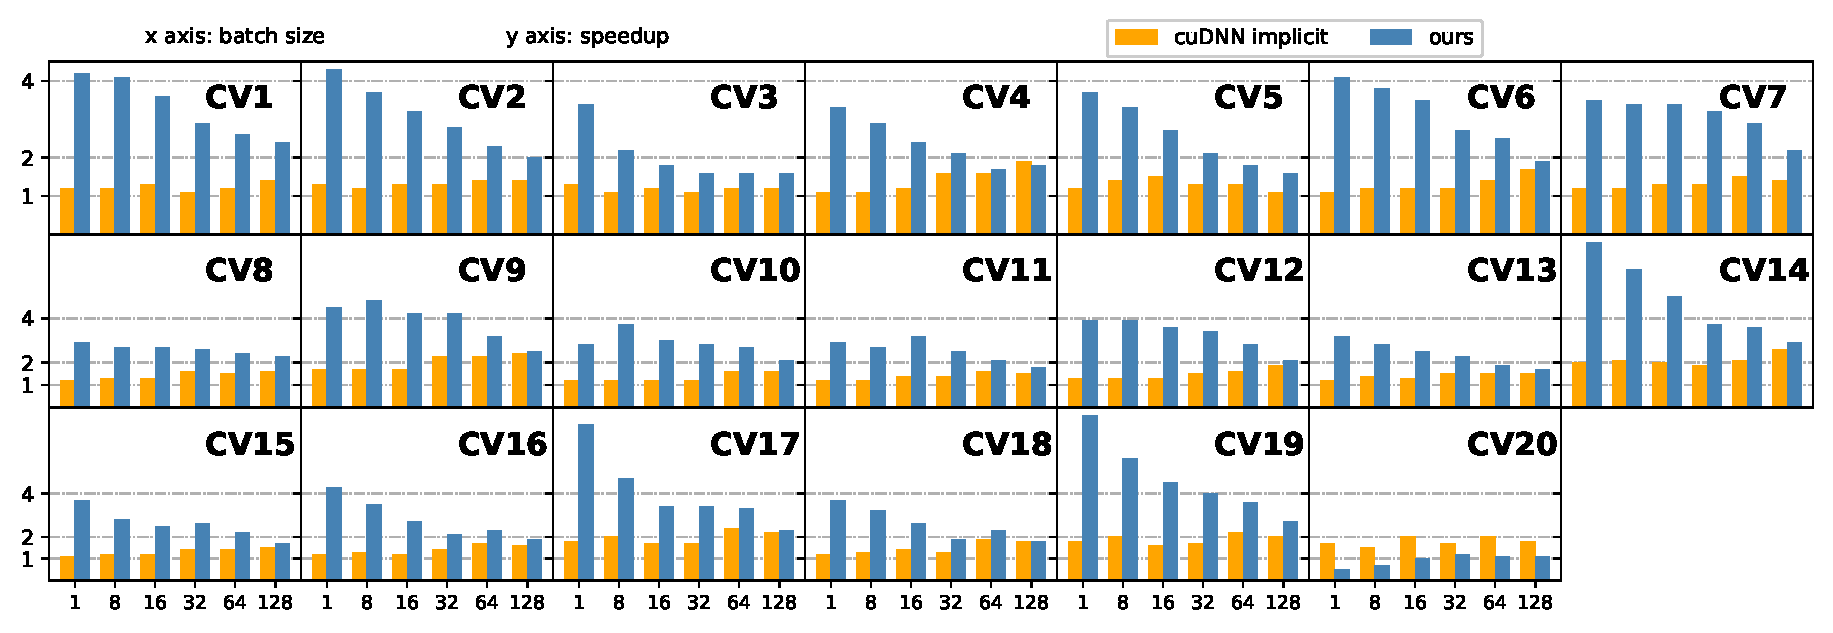
\includegraphics[width=\textwidth,height=6.2cm]{./figure/pwspeeduprtx.eps}
	\label{fig:pwspeeduprtx}}
\vspace{-5mm}
	\subfloat[]{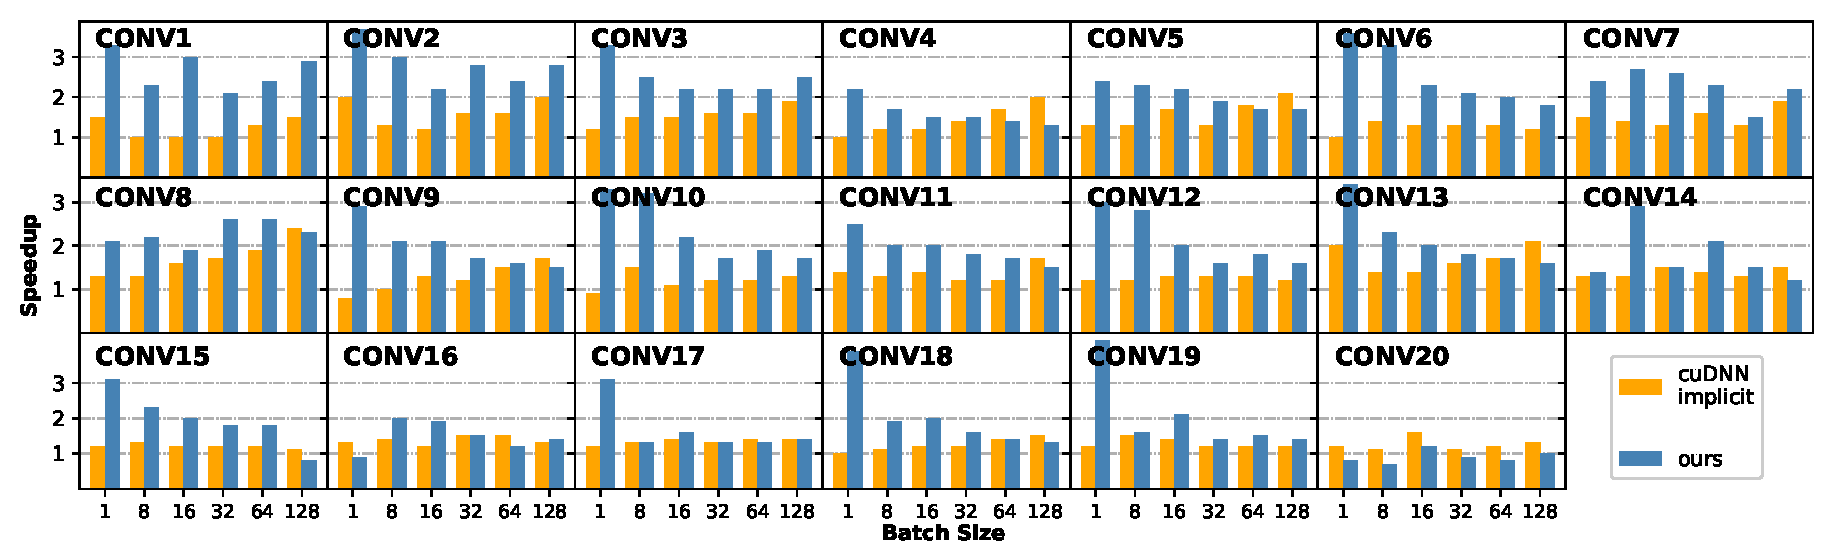
\includegraphics[width=\textwidth,height=6.2cm]{./figure/pwspeedupjetson.eps}
	\label{fig:pwspeedupjetson}}
	\vspace{-6mm}
	\caption{Speedups of cuDNN implicit and ours over cuDNN gemm for pointwise convolutions with FP32 on two platforms. Above: speedups on 2080Ti. Below: speedups on Xavier.}
	\label{fig:pwspeedupfp32}
\end{figure*}

\begin{figure*}
\captionsetup[subfloat]{labelformat=empty,skip=0pt}

	\centering
	\subfloat[]{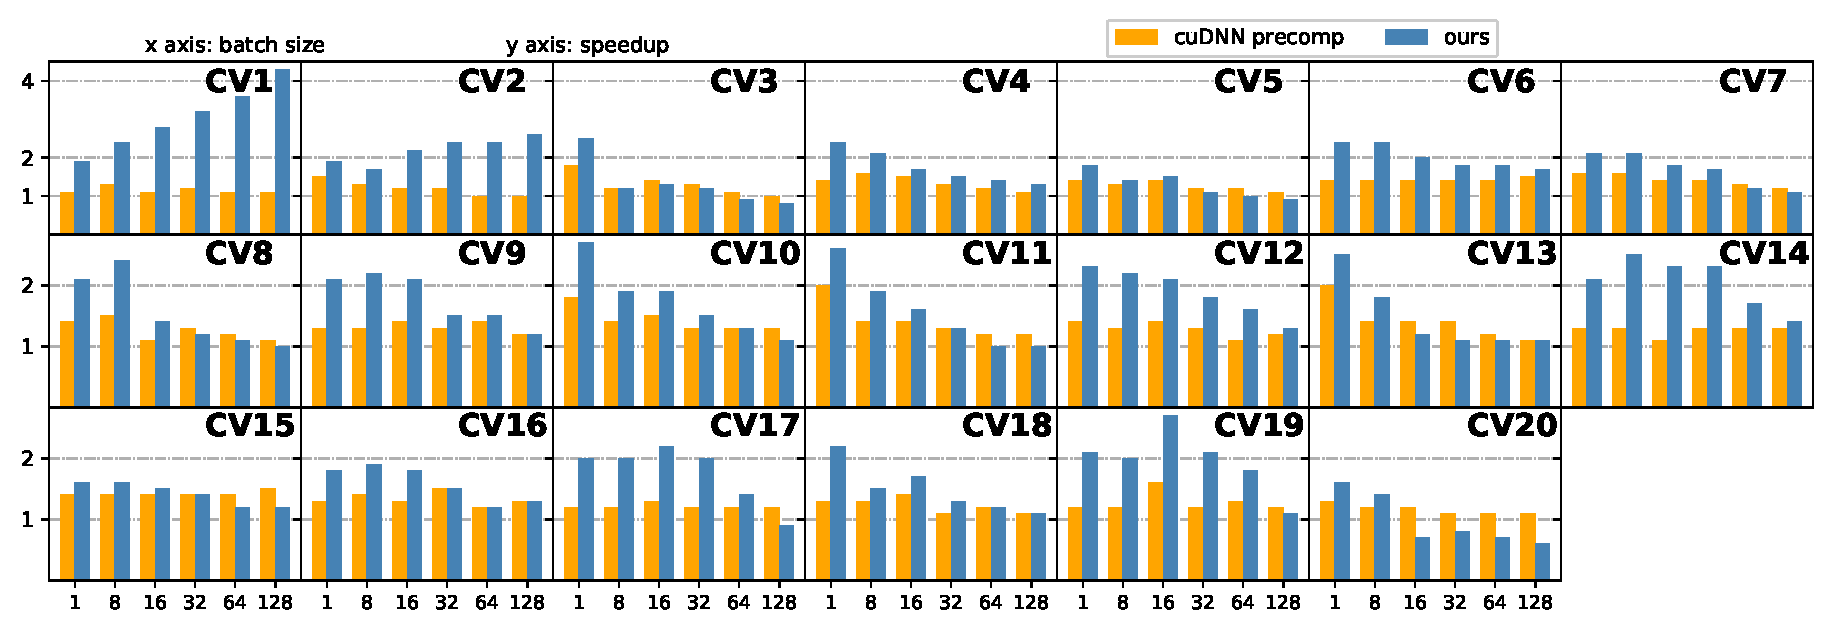
\includegraphics[width=\textwidth,height=6.2cm]{./figure/pwspeeduprtxint8.eps}
	\label{fig:pwspeeduprtxint8}}
	\vspace{-5mm}
	\subfloat[]{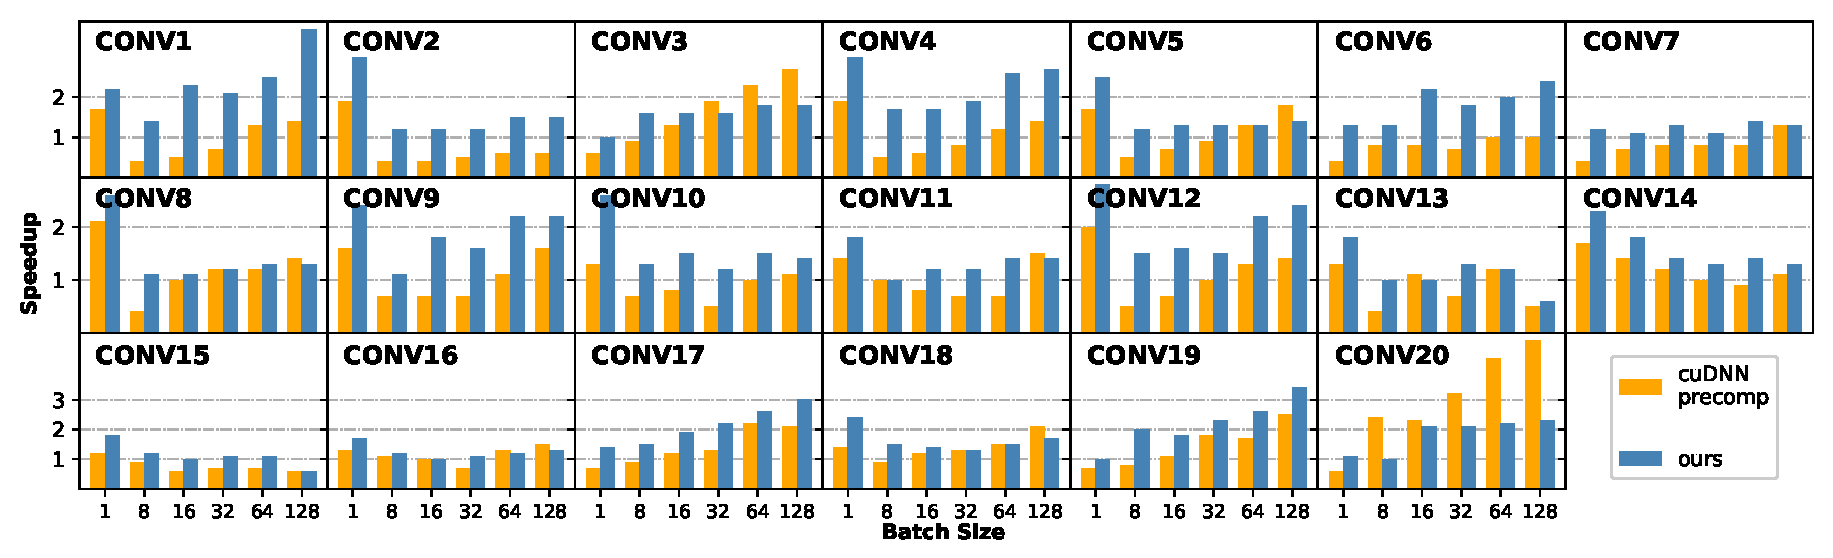
\includegraphics[width=\textwidth,height=6.2cm]{./figure/pwspeedupjetsonint8.eps}
	\label{fig:pwspeedupjetsonint8}}
	\vspace{-6mm}
	\caption{Speedups of cuDNN precomp and ours over cuDNN implicit for pointwise convolutions with INT8 on two platforms. Above: speedups on 2080Ti. Below: speedups on Xavier.}
	\label{fig:pwspeedupint8}
\end{figure*}

%\begin{figure}
%\centering
%	
%\subfloat{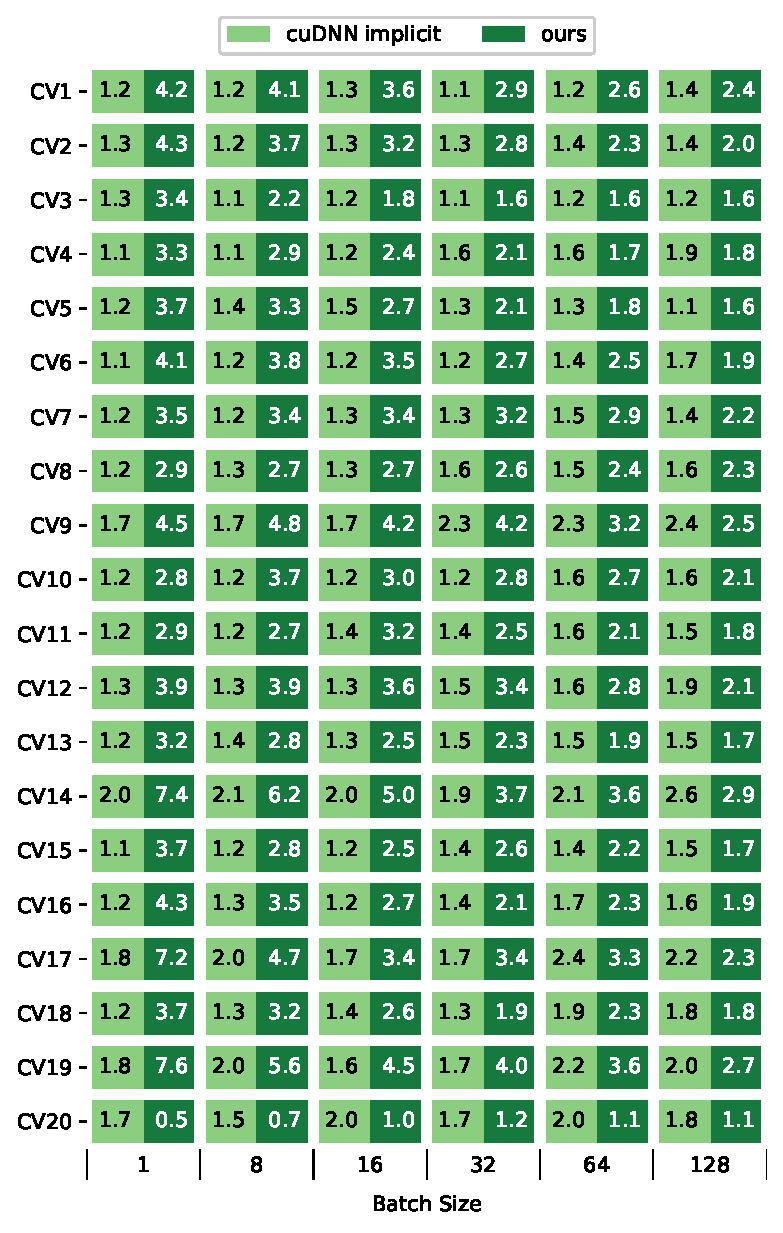
\includegraphics[width=\columnwidth,height=13cm]{./figure/pwexectime.eps}}
%\vspace{-2mm}
%\caption{Speedups of cuDNN implicit and our approach over cuDNN gemm} \label{fig:pwexectime}
%\vspace{-5mm}
%\end{figure}


\subsubsection{Setup} In this experiment, we compare our approach against all available pointwise convolution implementations in cuDNN.
The execution time of our approach includes both CPU and GPU parts, as shown in Algorithm \ref{algo:pwalgo}.
We use the layer configurations from the popular CNN model MobileNetv2.
There are 30 different configurations for pointwise convolution, we test all configurations and report the performance of 20 layers.
The other 10 layers exhibit similar performance as the selected ones.
We report the performance when batch sizes are set to 1, 8, 16, 32, 64 and 128.

When using data type FP32, cuDNN implicit performs best among all algorithms in cuDNN, therefore we only show results of cuDNN implicit and take cuDNN gemm as the baseline implementation.
When using data type INT8, cuDNN precomp performs best, therefore we show results of cuDNN precomp and take cuDNN implicit as the baseline.
Table \ref{tab:pwconv} lists the layer configurations used in this experiment.

\subsubsection{Overall results} Figure \ref{fig:pwspeedupfp32} shows speedups of cuDNN implicit and our approach over cuDNN gemm for pointwise convolutions with FP32 on two platforms.
Our approach achieves the best performance for layers of CV1-CV19.
For the layer CV20, which uses 1024 filters to convolve with the input, our approach performs poorly compared to cuDNN gemm and cuDNN implicit.
Overall, our implementation and cuDNN implicit achieve an average speedup of $3\times$ and $1.5\times$ over cuDNN gemm on 2080Ti respectively, and $2\times$ and $1.3\times$ on Xavier respectively.
This translates to an improvement of $2\times$ and $1.5\times$ over cuDNN implicit on 2080Ti and Xavier respectively.

Figure \ref{fig:pwspeedupint8} shows speedups of cuDNN precomp and our approach over cuDNN implicit for pointwise convolutions with INT8 on two platforms.
On 2080Ti, our approach and cuDNN precomp achieve an average speedup of $1.7\times$ and $1.3\times$ respectively.
On Xavier, our approach and cuDNN precomp achieve an average speedup of $1.6\times$ and $1.2\times$ respectively.
In summary, our approach obtains $1.3\times$ and $1.5\times$ speedup over cuDNN precomp on 2080Ti and Xavier respectively.


\subsubsection{Further analysis}
\begin{figure}
    \centering
    \subfloat[][SM utilizations of cuDNN implicit and our approach.]{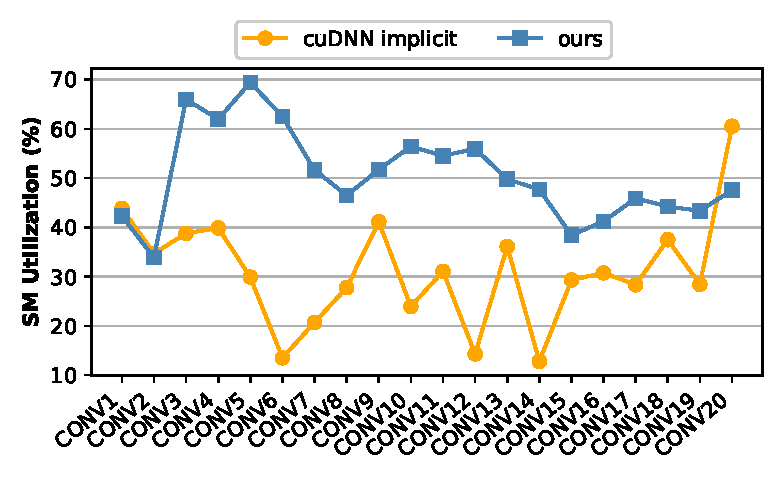
\includegraphics[width=\columnwidth]{./figure/pwsmutil.eps}\label{fig:pwsmutil}}
    \qquad

    \subfloat[][Ratios of executed LDG (load from global memory) instruction counts of cuDNN implicit to our approach.]{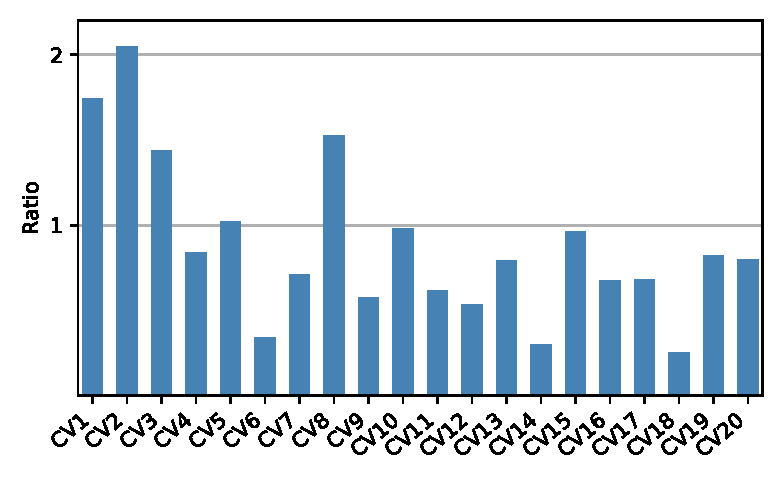
\includegraphics[width=\columnwidth]{./figure/pwldginst.eps}\label{fig:pwldginst}}
    \vspace{-2mm}
    \caption{SM utilizations and ratios of executed LDG instruction counts for pointwise convolutions with a batch size of 32 on 2080Ti.}
    \label{fig:pwinfo}
\end{figure}
Figure \ref{fig:pwinfo} reports the measured SM utilizations and ratios of executed LDG instruction counts of cuDNN implicit to our approach when using a batch size of 32 on 2080Ti. Other configurations have the similar performance.

Given a specific layer configuration of pointwise convolution, our approach will try to create a suitable number of thread blocks to saturate GPU.
A potential performance issue is that more thread blocks may incur more reloads of filters or inputs which are shared between thread blocks.
As shown in Figure \ref{fig:pwldginst}, our approach needs more than $2\times$ LDG instructions than cuDNN implicit in some cases.
In contrary to memory performance, the overall performance of our approach is $2\times$ faster than cuDNN implicit.
There are two reasons for the performance gain of our approach.
\begin{enumerate}
	\item Our approach exhibits a much higher SM utilization than cuDNN implicit.
	We can see in Figure \ref{fig:pwsmutil} that our approach has an average of $1.9\times$ higher SM utilization compared to cuDNN implicit.
	When executing pointwise convolution with a batch size of 128 or below, cuDNN implicit can not utilize SMs efficiently because of its fixed block size.
	Based on our dynamic block size method, we improve SM utilization which leads to performance improvement for pointwise convolution.
	\item We use a double buffer and multiple accumulations of output to hide memory access latency.
	Figure \ref{fig:stalllongscore} shows the average number of cycles each warp spends on waiting for the global operation to complete.
	We implement a simple pointwise without latency hiding, denoted as simple.
	We can see that our approach can significantly reduce the memory access latency compared to the simple implementation.
	To further reduce memory access latency, we need assembly level optimizations which is not the focus of this work.
\end{enumerate}

We observe some performance degradation for pointwise convolutions with INT8 data type.
When performing pointwise convolutions with INT8, we use $NHWC$ data format and four continuous INT8 channels can be viewed as an INT32 channel.
Thus, the size of channel dimension is reduced to one fourth of the original size.
For small channel sizes ($I_C \leq 96$), the corresponding reduced channel sizes restrict  choices of the number of distributed channels, which may lead to suboptimal performance compared to original channel sizes.

\subsubsection{Summary} We use dynamic block size method to improve SM utilization and use a double buffer and multiple accumulations to hide memory access latency. With both methods, we achieve an average speedup of $2\times$ and $1.5\times$ over cuDNN implicit on 2080Ti and Xavier respectively.


\begin{figure*}
    \centering
    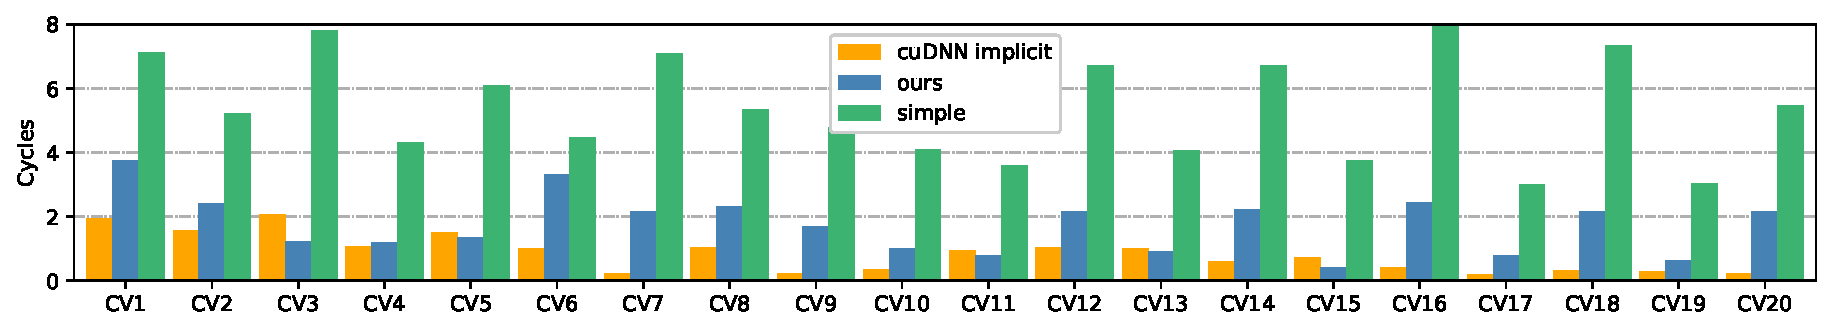
\includegraphics[width=0.97\textwidth,height=3cm]{./figure/longscore.eps}
    \caption{The average number of cycles each warp spends on waiting for the global memory access to complete.}
    \label{fig:stalllongscore}
\end{figure*}

\subsection{Inference and Training Performance}
\label{sec:inferexp}
\subsubsection{Setup}
In this experiment, we apply our depthwise and pointwise convolutions to MobileNetV2 and report the performance of inference and training.

For inference, we test normal and quantized MobileNetV2 with batch sizes of 1, 8, 16, 32, 64 and 128 on both platforms and report the inference time.
When applying quantization to pointwise convolutions, the input and filter are quantized from FP32 to INT8 and the output is still FP32.
Since cuDNN performs poorly for depthwise convolutions with INT8, we do not apply quantization to  depthwise convolutions.
Other operations are quantized normally.

For training, we test MobileNetV2 with batch sizes of 16, 32, 64 and 128 on 2080Ti and report the average training time of one iteration including one forward phase and one backward phase.

We use the caffe framework to implement MobileNetV2 and replace the implementations of batchnormalization and depthwise convolution layers of caffe with cuDNN implementations.
To experiment, we first run the inference with cuDNN implementation, denoted as \textbf{cuDNN}, and then replace the cuDNN with our implementations, denoted as \textbf{Ours}.
We also report the improvement of our approach compared to cuDNN implementations, denoted as \textbf{Improve}.

\subsubsection{Overall result}
\begin{table}[]
\setlength{\tabcolsep}{4.4pt}
    \caption{Inference time of MobileNetV2 with FP32 and INT8 on 2080Ti and Xavier}
    \vspace{-3mm}
    \label{tab:infertime}
    \centering
    %\rowcolors{2}{}{Gray}
    \begin{threeparttable}
    \begin{tabular}{c|l|rrrrrr}
    \toprule
    &\textbf{Batch} & 1 & 8 & 16& 32 &64 & 128\\
    \midrule
    %normal MobileNetV2
    \multirow{3}{*}{\textbf{\shortstack{2080Ti\\(FP32)}}}
    &\textbf{cuDNN (ms)}   &7.5  &8.8  &9.7  &14.4 &19.1 &28.7 \\
    &\textbf{Ours (ms)}    &6.1  &7.1  &8.0  &12.0 &16.9 &26.3\\
    &\textbf{Improve (\%)} &18.6 &19.3 &17.5 &16.7 &11.5 &8.4 \\
    \hline
    \multirow{3}{*}{\textbf{\shortstack{Xavier\\(FP32)}}}
    &\textbf{cuDNN (ms)}   &16.6 &22.3 &32.1 &52.6 &84.2 &140.1  \\
    &\textbf{Ours (ms)}    &13.2 &18.9 &27.8 &44.7 &76.1 &130.0 \\
    &\textbf{Improve (\%)} &20.5 &15.2 &13.4 &15.0 &9.6  &7.2 \\
    \hline
    %quantized MobileNetV2
    \multirow{3}{*}{\textbf{\shortstack{2080Ti\\(INT8)}}}
    &\textbf{cuDNN (ms)}   &6.3  &7.4  &7.7  &11.2 &14.6 &20.2 \\
    &\textbf{Ours (ms)}    &5.5  &6.6  &6.8  &10.3 &14.0 &19.7\\
    &\textbf{Improve (\%)} &12.7 &10.8 &11.7 &8.0  &4.1  &2.5 \\
    \hline
    \multirow{3}{*}{\textbf{\shortstack{Xavier\\(INT8)}}}
    &\textbf{cuDNN (ms)}   &13.3 &18.0 &27.0 &42.6 &64.8 &103.7  \\
    &\textbf{Ours (ms)}    &11.7 &15.4 &22.7 &38.8 &58.3 &94.4 \\
    &\textbf{Improve (\%)} &12.0 &14.4 &16.0 &8.9 &10.0  &9.0 \\


    \bottomrule
    \end{tabular}
    \footnotesize
    \end{threeparttable}

\end{table}

\begin{table}[]

    \caption{Training time of MobileNetV2 with FP32 on 2080Ti}
    \vspace{-3mm}
    \label{tab:traintime}
    \centering
    %\rowcolors{2}{}{Gray}
    \begin{threeparttable}
    \begin{tabular}{c|l|rrrr}
    \toprule
    &\textbf{Batch} & 16& 32 &64 & 128\\
    \midrule
    \multirow{3}{*}{\textbf{2080Ti}}&\textbf{cuDNN (ms)} & 16.6 & 27.6 & 43,4 &75.4 \\
    &\textbf{Ours (ms)} & 14.5  &24.1 &39.9 &71.3\\
    &\textbf{Improve (\%)} &12.7  &12.7 &8.1 &5.4 \\
    \bottomrule
    \end{tabular}
    \footnotesize
    \end{threeparttable}
    \vspace{-5mm}
\end{table}
Table \ref{tab:infertime} demonstrates the performance of inference.
For MobileNetV2 with FP32, our approach improves the performance of inference by 12.2\% and 13.5\% on average compared to the implementation of cuDNN implicit on 2080Ti and Xavier respectively.
For MobileNetV2 with INT8, we obtain 8.5\% and 11.7\% improvements on average over cuDNN precomp on 2080Ti and Xavier respectively.
Table \ref{tab:traintime} demonstrates that our approach improves the performance of training by 9.7\% on average compared to the implementation of cuDNN implicit on 2080Ti.
